\section{Perforator первой версии}
В рамках данной работы проводилась разработка системы распределенного анализа производительности приложений на масштабах целых датацентов.
Система носит рабочее название <<Perforator>>.

\subsection{Архитектура}
В начале разработки требовалось за наиболее короткое время получить рабочий прототип,
позволяющий регулярно собирать актуальные профили с промышленных окружений и проводить
оптимизации реальных программ. Для решения была выработана следующая архитектура:

\begin{itemize}
    \item
        Централизированный микросервис <<Scraper>> получает профили с заранее настроенного списка сервисов.

    \item
        Каждый полученный профиль аннотируется дополнительными метками, такими как имя хоста и модель CPU, после чего записывается в общее хранилище профилей.

    \item
        Хранилище профилей реализовано поверх широко используемой внутри Яндекса системы хранения и обработки данных YTsaurus \cite{yt}.

    \item
        Для изучения профилей разработчиками был написан достаточно примитивный веб-интерфейс, позволяющий смотреть список профилей
        в порядке появления по конкретным сервисам и по всей системе.

    \item
        Профили регулярно удаляются из системы: разработчикам интересны актуальные профили.
        При этом, поддержана возможность сохранять некоторые профили (те, что изучали разработчики) на значительно большее время.

    \item
        В настоящее время в системе не поддержана агрегация профилей по различным измерениям.
        Например, нельзя построить профиль по всему сервису за день или профиль по конкретному хосту.

\end{itemize}

Рассмотрим основные компоненты системы подробнее.

\begin{figure}[H]
    \centering
    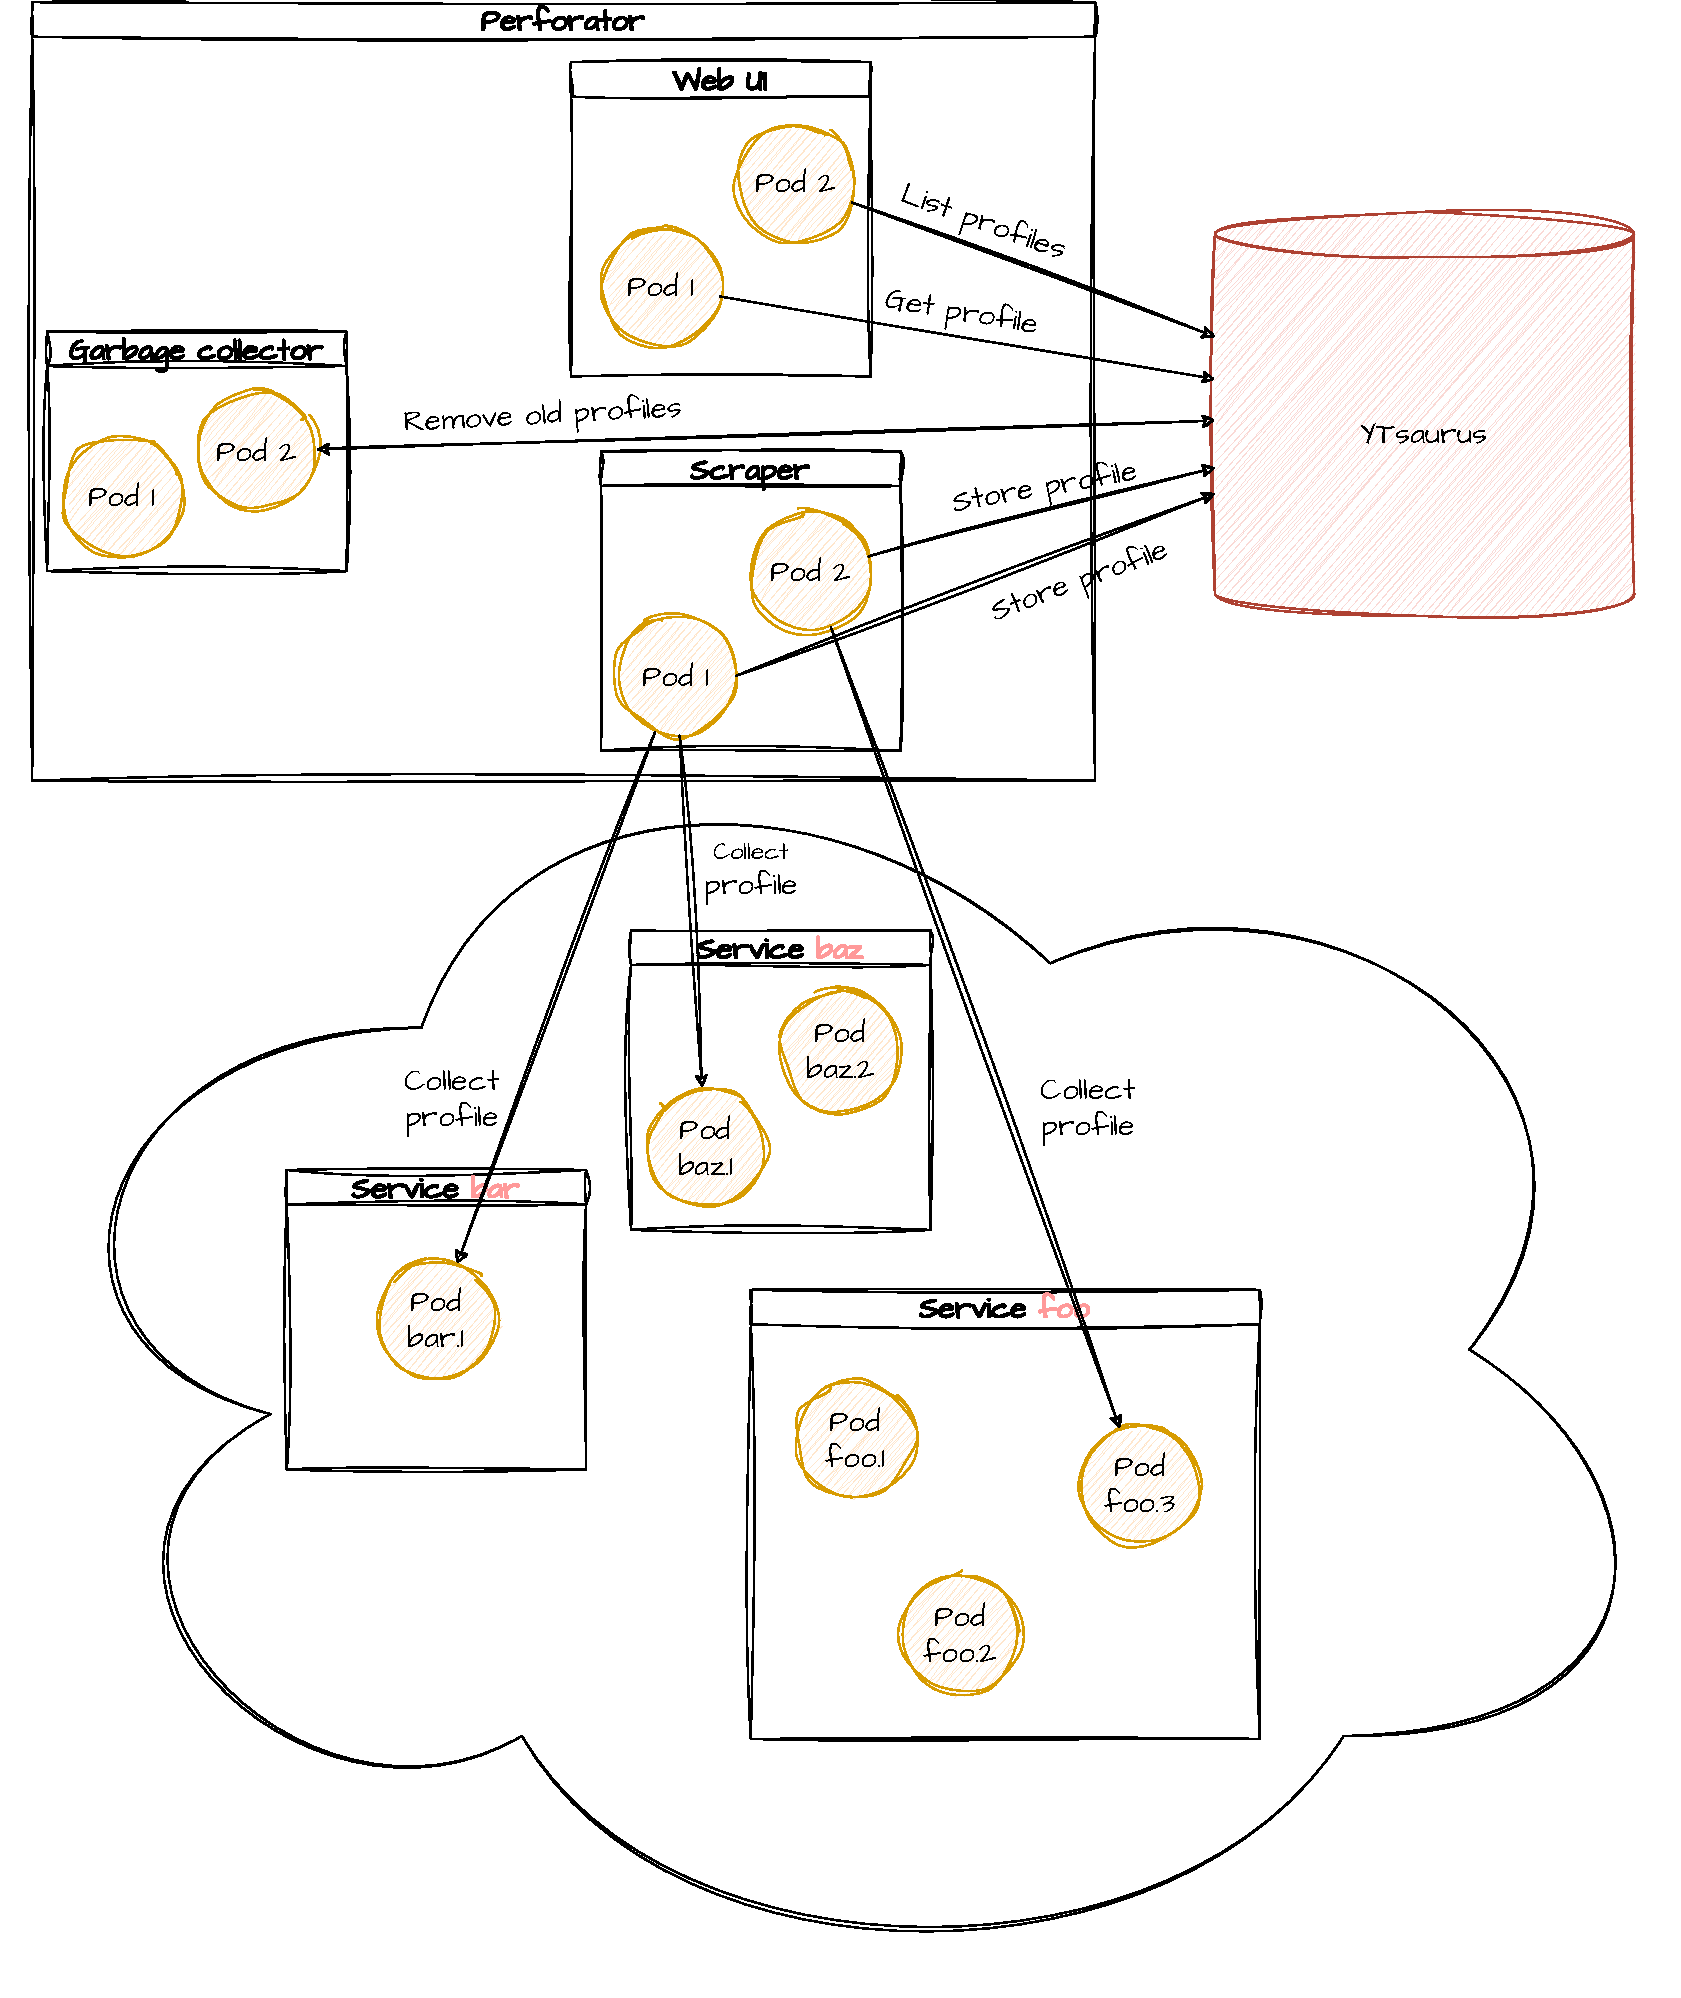
\includegraphics[width=\textwidth]{perforator.pdf}
    \caption{Схема первой версии сервиса}
    \label{fig:simple}
\end{figure}

\subsubsection{Сборщик профилей}
Scraper проходится по каждому сервису, подключается к нему одним из поддержанных способов (по HTTP, через SSH) и собирает профиль.
В настоящее время основным способом подключения сервиса является настройка доступа Scraper к хостам сервиса через SSH.
В этом режиме Scraper использует perf для сбора профиля по CPU cycles.
После сбора профиля на каждом хосте perf символизирует профиль, превращая адреса инструкций в имена функций.
Результат работы perf конвертируется в формат pprof: стандартный для большого количества современных семплирующих профилировщиков
формат, используемый в pprof и gperftools.

Подавляющее большинство сервисов, анализируемых Scraper, запущены в контейнерах под управлением системы контейнеризации Porto \cite{porto}.
Scraper анализирует конкретные процессы, определяемые по заданным пользователями правилам:
например, слушающие на определенном TCP порту или имеющим строку запуска, удовлетворяющую регулярному выражению.

Типичное время сбора профиля – минута на частоте около 500 Hz (десятки тысяч семплов), типичный размер сжатого профиля – 5 MiB.
В теории сервис не ограничен видом анализируемой метрики, профили могут быть произвольной природы.
В частности, тривиально поддерживются различные виды системных метрик, доступных подсистеме Linux perf.
На практике подавляющее большинство профилей собирается семплированием тактов процессора.

По результатам анализа не было выявлено сколько-нибудь значимого эффекта при включении perf на продуктовых процессах,
включая самые чувствительные к задержкам.

Для защиты от потенциальных проблем Scraper анализирует не все хосты сервиса, а небольшое статически выбираемое подмножество.
Это позволяет гарантировать, что в случае проблем с реализацией Perforator, perf или ядра Linux профилирования не нанесет значительного
вреда сервису.

Благодаря pull модели (сервис сам забирает профили с системы), автоматически поддержана возможность собирать профили с встроенных
в программу библиотек профилирования, таких как \lstinline!net/http/pprof! \cite{golang:pprof} в Golang.

\subsubsection{Хранилище профилей}
Хранилище профилей реализовано поверх широко используемой внутри Яндекса системы хранения и обработки данных YTsaurus \cite{yt}.
Хранилище разбито на две \textit{динамических таблицы} (OLTP KV хранилище в терминах YTsaurus).

Легковесная таблица метаинформации хранит нужную для обработки и поиска информацию о профиле: с какого хоста он снят, в какое время.
Данная таблица находится целиком в памяти, доступ к ней дешевый и эффективный,
это позволяет использовать тяжелые full-scan запросы при работе с ней.

Тяжелая таблица профилей содержит собственно профили, запросы туда исключительно легкие для системы: выбор профиля по ключу
(LookupRows в терминах YTsaurus). Кроме того, вместо данной таблицы поддержана возможность организации хранилища при помощи
Amazon S3-совместимого провайдера.
В этом режиме использование специализированной для хранения тяжелых данных системы позволяет сэкономить диск и снизить расходы
на чтение и запись профилей. При использовании динамических таблиц тяжелые профили неизбежно проходят через протокол консенсуса.

\subsubsection{Визуализация}
Для изучения профилей разработчиками был написан достаточно примитивный веб-интерфейс с использованием
UI-фреймворка Bootstrap \cite{bootstrap}, позволяющий смотреть список профилей
в порядке появления по конкретным сервисам и по всей системе.
Профили визуализируются в формате Flamegraph.

При разработке сервиса был реализован код отрисовки flamegraph, так как оригинальный код Brendan Gregg \cite{flamegraph}
не отличался большой производительностью: на отрисовку flamegraph по одному профилю в несколько мегабайт тратилось несколько минут.
Скрипт был переписан на Golang и дополнительно оптимизирован, что позволило ускорить отрисовку в десятки раз.

Кроме того, было найдено несколько ошибок в данном крайне популярном инструменте, один из которых был критичным.
При анализе результата работы perf flamegraph не учитывал веса семплов.
Это приводило к появлению на профиле большого количества (вплоть до 30\%) функций переключения контекста в ядре операционной
системы. При переключении контекста необходимо обновить состояние PMU, и современные процессоры при переключении
генерируют большое количество прерываний с нулевым весом.

Данная проблема была найдена несколькими независимыми разработчиками.
Стороннее решение появилось \cite{flamegraph:weight} вскоре после обнаружения в данном проекте.

\subsubsection{Сборка мусора}
Профили регулярно удаляются из системы: разработчикам интересны актуальные профили.
Выбрана экспоненциально затухающая политика хранения профилей с настраиваемым периодом полураспада профиля.
При этом, поддержана возможность сохранять некоторые профили (те, что изучали разработчики) на значительно большее время.

\subsubsection{Продвинутые возможности}
Система поддерживает возможность анализа конкретного хоста сервиса по запросу пользователя.
Это позволяет точечно анализировать проблемые хосты, не дожидаясь, пока Scraper случайным образом выберет их.

\subsection{Внедрение}
Первая версия системы была разработана и внедрена в сжатые сроки.
Легкий доступ к большому количеству актуальных профилей позволил разработчикам быстро устранять узкие места,
что привело к суммарному объему оптимизаций порядка десятков тысяч процессорных ядер.
Экспериментально было подтверждено эмпирическое наблюдение, что профиль программы под нагрузкой часто сильно отличается от профиля в
спокойном состоянии. Для некоторых сервисов различие настолько велико, что для оптимизации пропускной способности имеет
смысл рассматривать исключительно предкритическое состояние под нагрузкой.

\subsection{Ограничения}
Описанная система отличается простотой реализации, что неизбежно приводит к значительным ограничениям:

\begin{itemize}
    \item
        Одной из самых больших проблем является необходимость ручной настройки системы для каждого сервиса.
        Владелец сервиса должен выдать доступ Scraper по SSH и явно прописать свой сервис в конфигурации Perforator.

    \item
        Использование perf в качестве основного инструмента профилирования приводит к не менее серьезным ограничениям.
        Все анализируемые сервисом программы должны быть собраны с директивой компилятора, запрещающим опускать пролог и эпилог функций.
        Это позволяет быстро раскручивать стеки через perf, однако требует нетривиальной настройки со стороны владельцев сервисов, и,
        потенциально, приводит к потери производительности.

        В качестве альтернативы пользователи могут включать особые режимы сбора стеков через perf: с использованием DWARF или
        LBR \todo{Last Branch Record (особый механизм в процессорах Intel, запоминающий несколько последних инструкций ветвления).}
        К сожалению, оба механизма недостаточно хорошо показывают себя на реальных задачах.
        Раскрутка через DWARF крайне тяжелая (каждый семпл копирует большой регион стека процесса из kernel space в user space).
        Оба варианта работают эвристически и часто теряют функции у основания стека из-за большой глубины стека в реальных программах
        (десятки и сотни функций).

    \item
        В настоящее время в системе не поддержана агрегация профилей по различным измерениям.
        Например, нельзя построить профиль по всему сервису за день или профиль по конкретному хосту.

    \item
        Pull схема плохо масштабируется. Scraper должен знать список всех серверов, где необходимо собирать профили.
\end{itemize}

С учетом вышеописанных проблем было принято решение о разработке значительно более сложной системы, призванной решить
все сложности простой схемы.
